%% Sections 3 (body), 4-6
The conclusions of an optimisation study are only as credible as the models it optimises.
Three verification levels were therefore applied before any design comparison was made.

\subsection{Closed-form benchmarks}

Table~\ref{tab:closedform} compares PyNite with closed-form solutions for a cantilever, a
fixed--fixed beam under uniform load, and a fixed-base portal frame under lateral load. The
portal solution follows from the slope-deflection method for inextensible members, with
$k = (I_b/L)/(I_c/h)$,
\begin{equation}
\Delta = \frac{Hh^3(2+3k)}{12EI_c(1+6k)},\qquad
M_{base} = \frac{Hh(1+3k)}{2(1+6k)},\qquad
M_{top} = \frac{3kHh}{2(1+6k)}.
\end{equation}
Agreement is at round-off level for the statically simple cases and within $10^{-5}$ for the
portal, the residual being the axial flexibility that PyNite includes. The second-order
response of a cantilever beam-column with axial load $P$ and tip load $H$ has the exact tip
sway $\Delta = \frac{H}{Pk}(\tan kL - kL)$, $k=\sqrt{P/EI}$. PyNite's P-$\Delta$ solver with
a single element is within 0.6\% of the exact value even at $P = 0.6P_{cr}$, and converges to
$<2\times10^{-6}$ with eight elements (Table~\ref{tab:closedform}), showing that its geometric
stiffness also captures the member (P-$\delta$) effect.

\begin{table}[!htbp]
\centering
\caption{PyNite versus closed-form solutions ($E = 200$~GPa).}
\label{tab:closedform}
\small
\fittable{\begin{tabular}{lrrr}
\toprule
Quantity & Closed form & PyNite & Rel. error \\
\midrule
Cantilever tip deflection (m) & 0.053333 & 0.053333 & 0.0e+00 \\
Cantilever fixed-end moment (kN m) & 200 & 200 & 0.0e+00 \\
Fixed beam end moment (kN m) & 213.33 & 213.33 & 4.0e-16 \\
Fixed beam mid-span moment (kN m) & 106.67 & 106.67 & 1.1e-15 \\
Fixed beam mid-span deflection (m) & 0.010667 & 0.010667 & 3.3e-16 \\
Portal sway (m) & 0.012698 & 0.012699 & 9.3e-06 \\
Portal column base moment (kN m) & 114.29 & 114.29 & 7.2e-06 \\
Portal column top moment (kN m) & 85.714 & 85.715 & 3.6e-06 \\
\midrule
\multicolumn{4}{l}{Second-order cantilever, tip sway (mm): exact vs PyNite P-$\Delta$ with $n$ elements} \\
$P/P_{cr}$ & exact & $n=1$ / $n=2$ / $n=8$ & err. ($n=1$, $n=8$) \\
0.2 & 25.972 & 25.964 / 25.972 / 25.972 & 3.3e-04, 1.0e-07 \\
0.4 & 34.534 & 34.471 / 34.529 / 34.534 & 1.8e-03, 5.5e-07 \\
0.6 & 51.650 & 51.326 / 51.627 / 51.650 & 6.3e-03, 1.8e-06 \\
\bottomrule
\end{tabular}}
\end{table}

\subsection{Independent solver}

The optimised designs were rebuilt in OpenSeesPy \citep{McKenna2010,Zhu2018} with
elastic beam-column elements, element loads for the distributed gravity and self-weight
and nodal storey forces, independently of the PyNite model. Table~\ref{tab:opensees} lists the
largest relative difference of each response quantity, normalised by the largest absolute value
of that quantity in the frame. For all five unit cases the two solvers agree to
$10^{-13}$--$10^{-16}$, i.e.\ to machine precision. (Gravity-load drifts of these symmetric
frames are themselves of the order of round-off and are not compared.) For the P-$\Delta$
analysis of the combination $1.2D+0.5L+1.6W$, OpenSees used the \texttt{PDelta} coordinate
transformation and a load-controlled Newton solution. PyNite's second-order drifts differ from
OpenSees by at most 0.8\%, and the $B_1$--$B_2$ amplified first-order drifts used by the
surrogate by at most 1.8\%, always on the conservative side (Fig.~\ref{fig:pdelta}); column
base moments behave similarly (at most 1.6\%).

\begin{table}[!htbp]
\centering
\caption{Maximum relative differences between PyNite and OpenSeesPy for the optimised base
designs and two other frames: linear unit cases and P-$\Delta$ analysis of $1.2D+0.5L+1.6W$.}
\label{tab:opensees}
\small
\fittable{\begin{tabular}{llrrrr}
\toprule
Design & Case & Drift & Column $M$ & Column $N$ & Beam end $M$ \\
\midrule
Base DDO & D & -- & 8.3e-16 & 2.0e-15 & 8.0e-16 \\
 & L & -- & 4.7e-16 & 1.6e-15 & 9.6e-16 \\
 & W & 1.8e-14 & 1.1e-14 & 9.8e-15 & 1.4e-14 \\
 & ND & 1.8e-14 & 1.3e-14 & 8.2e-15 & 1.4e-14 \\
 & NL & 1.5e-14 & 1.0e-14 & 8.7e-15 & 1.3e-14 \\
 & P-$\Delta$: PyNite & 7.3e-03 & 7.4e-03 & & \\
 & P-$\Delta$: $B_1$--$B_2$ & 1.8e-02 & 1.6e-02 & & \\
\midrule
Base RBDO-C & D & -- & 6.7e-16 & 1.4e-15 & 4.7e-16 \\
 & L & -- & 6.7e-16 & 1.3e-15 & 6.7e-16 \\
 & W & 4.2e-14 & 4.3e-14 & 3.0e-14 & 4.2e-14 \\
 & ND & 4.2e-14 & 4.2e-14 & 2.9e-14 & 4.1e-14 \\
 & NL & 4.2e-14 & 4.3e-14 & 3.0e-14 & 4.2e-14 \\
 & P-$\Delta$: PyNite & 7.1e-03 & 6.2e-03 & & \\
 & P-$\Delta$: $B_1$--$B_2$ & 1.5e-02 & 1.5e-02 & & \\
\midrule
3-storey DDO & D & -- & 3.1e-16 & 1.1e-15 & 4.9e-16 \\
 & L & -- & 7.7e-16 & 8.8e-16 & 5.5e-16 \\
 & W & 6.0e-15 & 6.9e-15 & 2.8e-15 & 4.0e-15 \\
 & ND & 6.0e-15 & 6.8e-15 & 2.9e-15 & 4.4e-15 \\
 & NL & 6.8e-15 & 7.4e-15 & 3.5e-15 & 4.4e-15 \\
 & P-$\Delta$: PyNite & 5.7e-03 & 6.2e-03 & & \\
 & P-$\Delta$: $B_1$--$B_2$ & 9.4e-03 & 1.5e-02 & & \\
\midrule
9-storey DDO & D & -- & 9.5e-16 & 2.0e-15 & 1.1e-15 \\
 & L & -- & 1.4e-15 & 2.8e-15 & 2.0e-15 \\
 & W & 1.7e-13 & 1.1e-13 & 1.3e-13 & 1.4e-13 \\
 & ND & 1.7e-13 & 1.2e-13 & 1.3e-13 & 1.4e-13 \\
 & NL & 1.7e-13 & 1.2e-13 & 1.3e-13 & 1.4e-13 \\
 & P-$\Delta$: PyNite & 8.1e-03 & 7.5e-03 & & \\
 & P-$\Delta$: $B_1$--$B_2$ & 1.8e-02 & 1.5e-02 & & \\
\bottomrule
\end{tabular}}
\end{table}

\begin{figure}[!htbp]
\centering
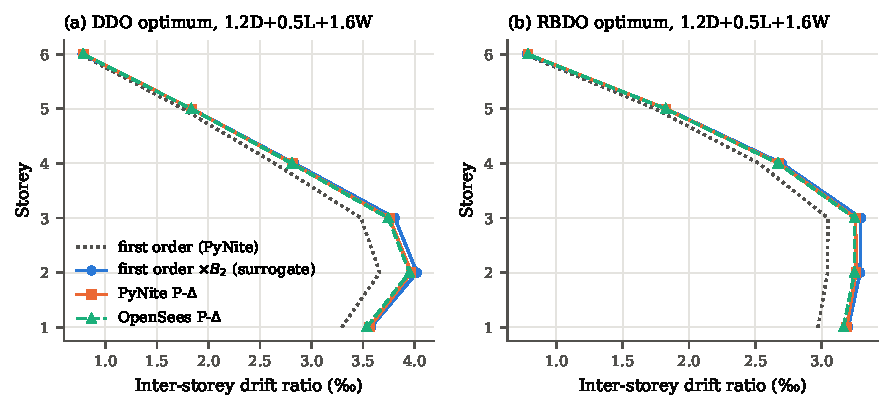
\includegraphics[width=\textwidth]{figures/pdelta.pdf}
\caption{Inter-storey drift profiles of the base designs under $1.2D+0.5L+1.6W$: first-order
PyNite, the $B_2$-amplified surrogate, PyNite P-$\Delta$ and OpenSees P-$\Delta$.}
\label{fig:pdelta}
\end{figure}

\subsection{Reliability surrogate versus full second-order re-analysis}

The surrogate rests on three simplifications: second-order effects through $B_1$--$B_2$, a
modulus that is uniform over the frame, and nominal section stiffness (the fabrication factor
enters the resistance only). To quantify their combined effect, 1000 samples of the wind
scenario $S_2$ were analysed for the base RBDO design with a full PyNite P-$\Delta$ analysis per
sample, in which every member received its own modulus factor (c.o.v.\ 0.03) and its
fabrication factor was applied to $A$ and $I$. The resulting system utilisation and maximum
drift ratio are compared with the surrogate evaluated on the same samples (with the mean of the
member modulus factors) in Fig.~\ref{fig:fullmc}. A second set of 1000 samples with the wind
doubled was added as a stress test that produces failure probabilities large enough to be
compared directly.

The surrogate overestimates the system utilisation by 0.9\% on average (standard deviation of
the difference 1.0\%, correlation 0.997) under $W_{50}$ and by 1.5\% under $2W_{50}$; the
corresponding failure fractions in the stress test are 2.1\% (surrogate) and 1.7\% (full
analysis). The drift ratio is unbiased ($-0.6\%$ mean difference, 2.0\% standard deviation) and
the drift exceedance fractions are 7.2\% and 7.1\%. The surrogate is thus slightly
conservative for the ULS and accurate for the drift SLS, while being two to three orders of
magnitude cheaper than a P-$\Delta$ re-analysis per sample.

\begin{figure}[!htbp]
\centering
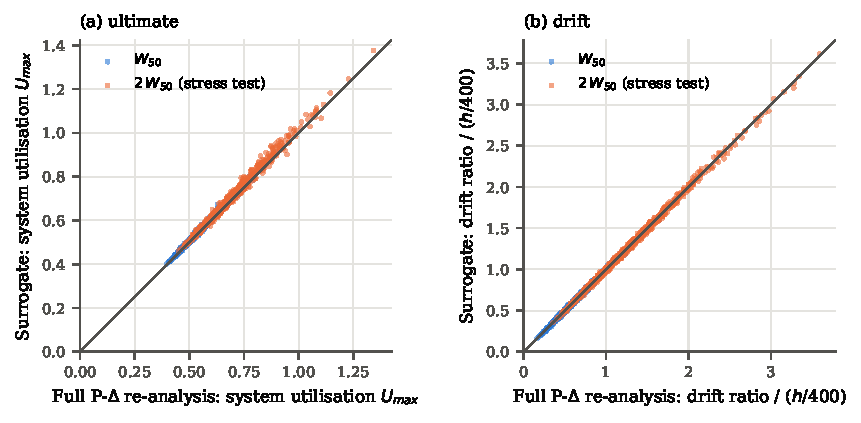
\includegraphics[width=\textwidth]{figures/fullmc.pdf}
\caption{Surrogate versus full P-$\Delta$ re-analysis with member-by-member random stiffness
and section properties (base RBDO design, 1000 samples per wind level).}
\label{fig:fullmc}
\end{figure}

\subsection{Monte Carlo convergence}

Fig.~\ref{fig:mcconv} shows the reliability indices of the base DDO and RBDO designs as
functions of the sample size for five independent random streams. At the SAA sample size
($N=5\times10^4$) the scatter of $\hat\beta_{ULS}$ between streams is about $\pm0.1$, which is
the resolution with which the optimiser can enforce $\beta_T=3$; at $N=10^6$ the streams agree
within $\pm0.02$ (c.o.v.\ of $\hat P_f$ about 3\%). The drift index converges much faster
because its failure probability is larger. These numbers justify the two-stage procedure of
Section~\ref{sec:mc}: the SAA estimate guides the search and the independent $10^6$-sample
estimate is the one reported.

\begin{figure}[!htbp]
\centering
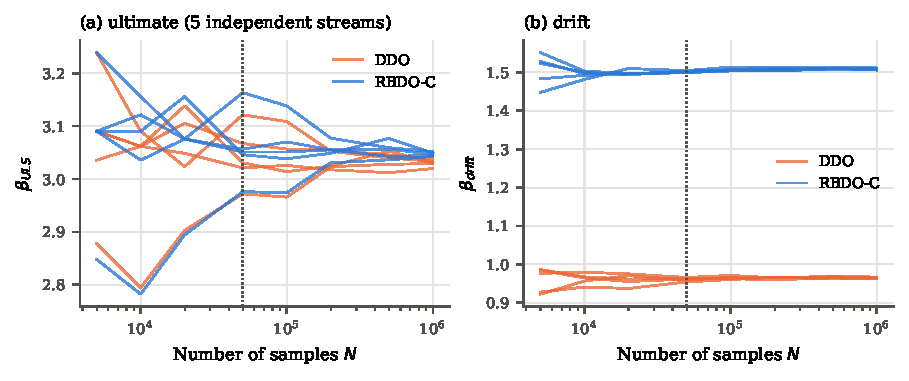
\includegraphics[width=\textwidth]{figures/mc_convergence.pdf}
\caption{Convergence of the Monte Carlo reliability indices of the base designs (five
independent streams each). The dotted line marks the SAA sample size used in the optimiser.}
\label{fig:mcconv}
\end{figure}

%% ---------------------------------------------------------------------------
\section{Results}\label{sec:results}

\subsection{Optimiser performance}

Table~\ref{tab:optruns} summarises the optimisation runs. Repeated DDO runs with different
seeds converged to the same design or to designs within 0.6\% in mass, and the two RBDO runs of
the base frame converged to the same design, which indicates that the GA with local search
reliably locates the optimum of these nine-variable problems (Fig.~\ref{fig:ga}). A DDO run
needs 6--12~min and an RBDO run 15--61~min on one CPU core, the reliability evaluation
accounting for about 80\% of the RBDO time.

\begin{table}[!htbp]
\centering
\caption{Optimisation runs (best design reported; spread = range of the best masses over the
seeds).}
\label{tab:optruns}
\small
\fittable{\begin{tabular}{llrrrr}
\toprule
Frame & Formulation & Runs & Best mass (kg) & Designs evaluated & Wall time (min) \\
\midrule
3 storeys & DDO & 2 & 7995 & 1556 & 2 \\
3 storeys & DDO-h450 & 1 & 7995 & 1652 & 2 \\
3 storeys & DDO-h500 & 1 & 7995 & 1652 & 2 \\
3 storeys & DDO-h600 & 1 & 7995 & 1652 & 2 \\
3 storeys & RBDO & 1 & 8188 & 1390 & 15 \\
3 storeys & RBDO-C & 2 & 8188 & 1346 & 10 \\
Base & DDO & 10 & 18261 & 2130 & 6 \\
Base & DDO-h450 & 1 & 18626 & 2175 & 6 \\
Base & DDO-h500 & 1 & 18787 & 2162 & 6 \\
Base & DDO-h600 & 1 & 20664 & 1967 & 5 \\
Base & RBDO & 2 & 18787 & 2074 & 44 \\
Base & RBDO-C & 5 & 18787 & 2109 & 31 \\
9 storeys & DDO & 2 & 32987 & 2247 & 12 \\
9 storeys & DDO-h450 & 1 & 34665 & 2196 & 8 \\
9 storeys & DDO-h500 & 1 & 35484 & 1938 & 8 \\
9 storeys & DDO-h600 & 1 & 38784 & 2177 & 8 \\
9 storeys & RBDO & 1 & 35450 & 1885 & 61 \\
9 storeys & RBDO-C & 2 & 35450 & 1950 & 47 \\
Bay 6 m & DDO & 2 & 13707 & 1937 & 6 \\
Bay 6 m & DDO-h450 & 1 & 14140 & 1758 & 4 \\
Bay 6 m & DDO-h500 & 1 & 14583 & 2105 & 6 \\
Bay 6 m & DDO-h600 & 1 & 15960 & 1952 & 5 \\
Bay 6 m & RBDO & 1 & 14621 & 2278 & 57 \\
Bay 6 m & RBDO-C & 2 & 14668 & 2220 & 38 \\
Bay 10 m & DDO & 2 & 25639 & 1938 & 7 \\
Bay 10 m & DDO-h450 & 1 & 26035 & 1936 & 5 \\
Bay 10 m & DDO-h500 & 1 & 26035 & 2154 & 5 \\
Bay 10 m & DDO-h600 & 1 & 27435 & 2260 & 5 \\
Bay 10 m & RBDO & 1 & 26065 & 2234 & 43 \\
Bay 10 m & RBDO-C & 2 & 26065 & 2080 & 32 \\
$p_w$ = 0.8 kPa & DDO & 2 & 17788 & 1999 & 6 \\
$p_w$ = 0.8 kPa & DDO-h450 & 1 & 17788 & 2128 & 5 \\
$p_w$ = 0.8 kPa & DDO-h500 & 1 & 17788 & 2128 & 5 \\
$p_w$ = 0.8 kPa & DDO-h600 & 1 & 18050 & 2230 & 5 \\
$p_w$ = 0.8 kPa & RBDO & 1 & 17874 & 2169 & 48 \\
$p_w$ = 0.8 kPa & RBDO-C & 2 & 17989 & 1979 & 32 \\
$p_w$ = 1.6 kPa & DDO & 2 & 19743 & 2153 & 7 \\
$p_w$ = 1.6 kPa & DDO-h450 & 1 & 20679 & 2098 & 5 \\
$p_w$ = 1.6 kPa & DDO-h500 & 1 & 21989 & 2240 & 6 \\
$p_w$ = 1.6 kPa & DDO-h600 & 1 & 23385 & 2221 & 5 \\
$p_w$ = 1.6 kPa & RBDO & 1 & 21738 & 2105 & 48 \\
$p_w$ = 1.6 kPa & RBDO-C & 3 & 21738 & 2103 & 34 \\
\bottomrule
\end{tabular}}
\end{table}

\begin{figure}[!htbp]
\centering
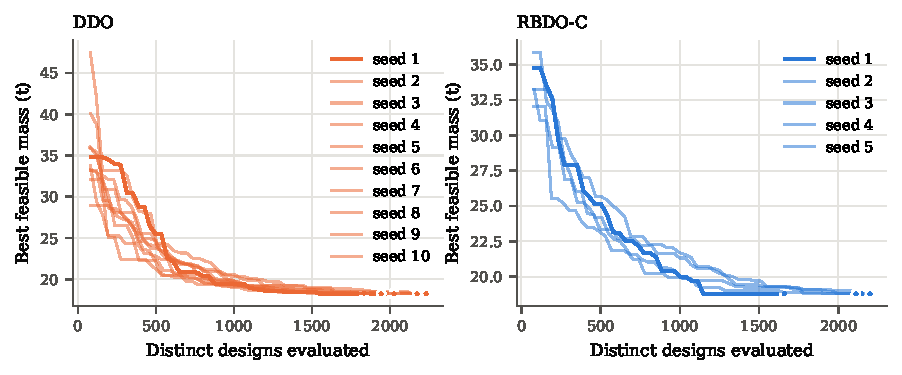
\includegraphics[width=\textwidth]{figures/ga_history.pdf}
\caption{Convergence of the GA for the base frame (best feasible mass); dots mark the final
designs after local search.}
\label{fig:ga}
\end{figure}

\subsection{Deterministic versus uncertainty-aware design of the base frame}

Table~\ref{tab:designs} compares the DDO and RBDO optima of the base frame. The DDO design
weighs 18.26~t; its governing LRFD ratio is 0.993 and its drift is 0.97 of the $h/400$ limit,
so both strength and drift are active. Verified with $10^6$ independent samples, its system
ULS reliability index is $\beta_{ULS}=3.03$, practically equal to the target, but its drift
reliability over 50 years is only $\beta_{drift} = 0.96$ ($P_f = 0.17$): a drift check at the
nominal 50-year wind leaves a one-in-six chance that the drift limit is exceeded during the
reference period. The reason is that the 50-year maximum wind has a mean-to-nominal ratio of
0.78 but a c.o.v.\ of 0.37, so the nominal wind is exceeded with a probability of about 0.19,
and serviceability checks carry no load factor.

The RBDO design ($\beta_T = 3.0$, $\beta_{SLS}=1.5$) weighs 18.79~t (+2.9\%) and achieves
$\beta_{ULS}=3.05$ and $\beta_{drift}=1.51$, i.e.\ both reliability constraints are active and
satisfied in the independent verification. The additional steel is placed where it buys
stiffness most cheaply: the lower-storey beams are deepened (W21$\times$50 to
W24$\times$55) and the interior columns of storeys 3--4 increased, while the remaining sections
are unchanged. Its deterministic drift ratio is 0.80 of $h/400$ (equivalent to $h/500$), and its
LRFD strength ratio decreases slightly to 0.977. The exceedance curves of Fig.~\ref{fig:exceed}
show that the two designs have virtually identical distributions of the system utilisation,
whereas the drift distribution of the RBDO design is shifted to the left over its whole range.

\begin{table}[!htbp]
\centering
\caption{Optimum designs of the base frame and their deterministic and probabilistic
performance (reliability indices from $10^6$ independent samples; $>$ indicates no failure in
the sample, i.e.\ a lower bound).}
\label{tab:designs}
\small
\fittable{\begin{tabular}{lllllll}
\toprule
 & \multicolumn{3}{c}{DDO} & \multicolumn{3}{c}{RBDO} \\
\cmidrule(lr){2-4}\cmidrule(lr){5-7}
Storeys & Ext. col. & Int. col. & Beam & Ext. col. & Int. col. & Beam \\
\midrule
1-2 & W14X61 & W14X90 & W21X50 & W14X61 & W14X90 & W24X55 \\
3-4 & W14X48 & W14X61 & W21X44 & W14X48 & W14X68 & W21X44 \\
5-6 & W14X48 & W14X48 & W21X44 & W14X48 & W14X48 & W21X44 \\
\midrule
Steel mass (t) & \multicolumn{3}{l}{18.26} & \multicolumn{3}{l}{18.79} \\
LRFD strength ratio & \multicolumn{3}{l}{0.993} & \multicolumn{3}{l}{0.977} \\
Drift ratio / limit (D+0.5L+W) & \multicolumn{3}{l}{0.972} & \multicolumn{3}{l}{0.798} \\
Deflection / limit (L) & \multicolumn{3}{l}{0.156} & \multicolumn{3}{l}{0.156} \\
Max. $B_2$ (DAM) & \multicolumn{3}{l}{1.186} & \multicolumn{3}{l}{1.151} \\
$\beta_{ULS}$ ($N=10^6$) & \multicolumn{3}{l}{3.03} & \multicolumn{3}{l}{3.05} \\
$P_{f,ULS}$ & \multicolumn{3}{l}{1.24e-03} & \multicolumn{3}{l}{1.15e-03} \\
$\beta_{drift}$ & \multicolumn{3}{l}{0.96} & \multicolumn{3}{l}{1.51} \\
$\beta_{defl}$ & \multicolumn{3}{l}{$>$4.89} & \multicolumn{3}{l}{$>$4.89} \\
\bottomrule
\end{tabular}}
\end{table}

\begin{figure}[!htbp]
\centering
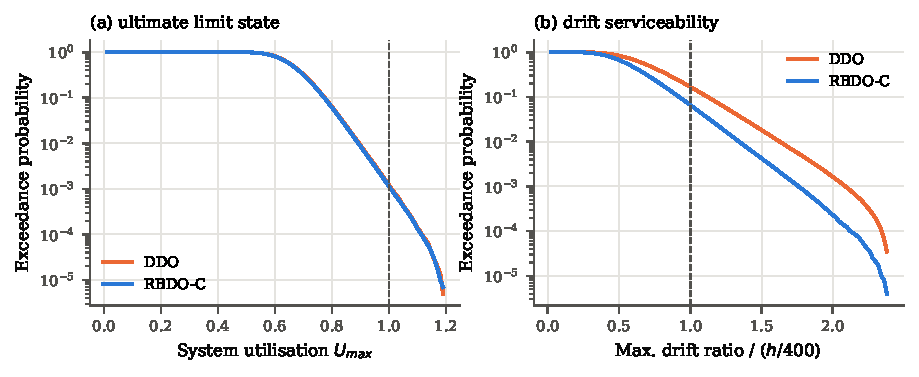
\includegraphics[width=\textwidth]{figures/exceedance.pdf}
\caption{Exceedance probabilities of the system utilisation (ULS) and of the maximum
inter-storey drift (normalised by $h/400$) of the base DDO and RBDO designs over 50 years
($10^6$ samples).}
\label{fig:exceed}
\end{figure}

Fig.~\ref{fig:memberutil} relates the member utilisations of the deterministic check to their
probabilistic counterparts. The 99.9\% quantile of the member utilisation lies 5--15\% below the
LRFD ratio for most members, which reflects the margin built into the partial factors. In
96\% of the failed samples of both designs the governing member is a beam, mostly at floor
levels 3--5 (79\% of failures for DDO, 96\% for RBDO), where the W21$\times$44 beams of the
upper storey groups are highly utilised; the remainder are exterior ground-storey columns and,
for DDO, first-floor beams. The gravity scenario $S_1$ with the 50-year live load causes 81\%
(DDO) and 96\% (RBDO) of the failures, which is consistent with the dominant influence of the
live-load c.o.v.\ found in the sensitivity study. Stiffening the frame against drift (RBDO)
therefore removes most wind-scenario failures without changing the gravity-governed ULS
reliability.

\begin{figure}[!htbp]
\centering
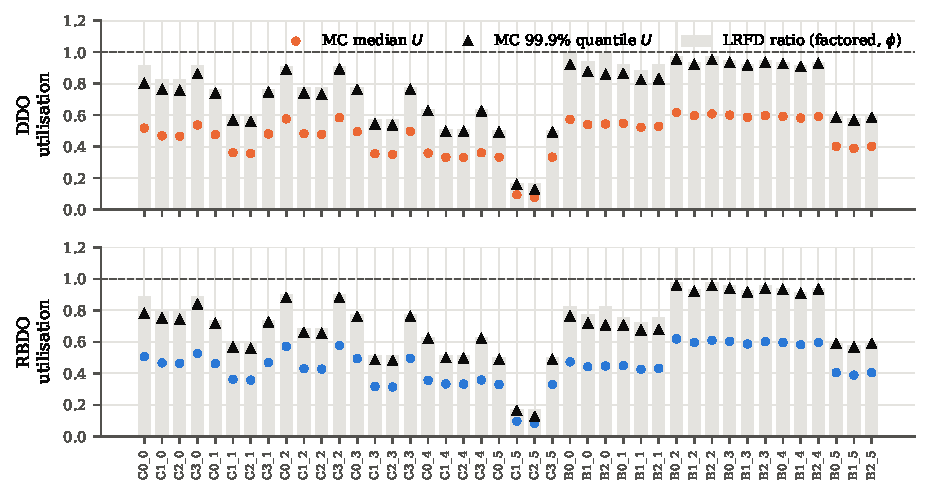
\includegraphics[width=\textwidth]{figures/member_util.pdf}
\caption{Member utilisations of the base designs: governing LRFD ratio (bars) and median and
99.9\% quantile of the probabilistic utilisation. Member labels: C$i\_s$ is the column on line
$i$ in storey $s$, B$i\_s$ the beam in bay $i$ at floor $s$ (counted from 0).}
\label{fig:memberutil}
\end{figure}

\subsection{Cost--reliability trade-off}

Fig.~\ref{fig:pareto} shows the non-dominated designs of the bi-objective problem (mass versus
$\beta_{ULS}$, subject to $\beta_{drift},\beta_{defl}\ge1.5$), re-verified with $4\times10^5$
independent samples, together with all feasible designs visited by NSGA-II. Because drift
governs the mass of this frame once $\beta_{SLS}=1.5$ is imposed, the front is almost vertical:
raising the ULS reliability from $\beta_{ULS}=3.06$ to 3.36, 3.64 and 3.83 costs only +1.3\%,
+3.5\% and +4.2\% of steel (19.04, 19.45 and 19.57~t against 18.79~t), whereas lowering it to
2.36 would save just 0.2\%. All front designs have $\beta_{drift}$ between 1.51 and 1.57
(Fig.~\ref{fig:pareto}b). The front passes through the single-objective RBDO optimum, which is
an independent check of both optimisers. The DDO optimum lies to the left of the front at a
similar $\beta_{ULS}$, but it does not belong to the feasible set because its
$\beta_{drift}=0.96$.

\begin{figure}[!htbp]
\centering
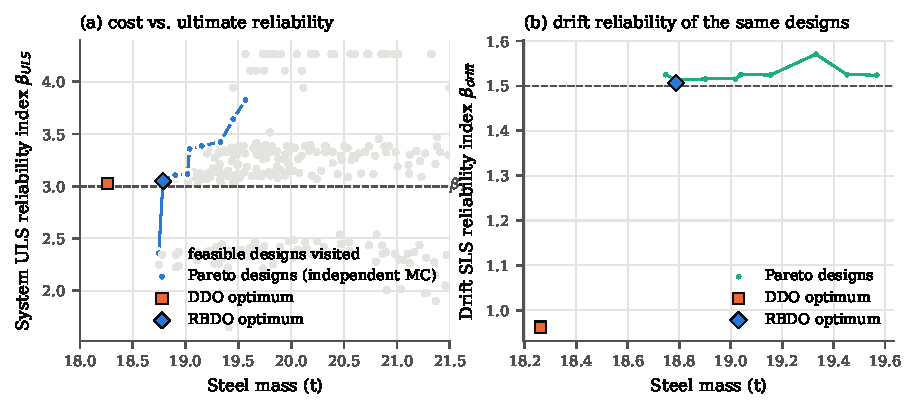
\includegraphics[width=\textwidth]{figures/pareto.pdf}
\caption{Cost--reliability trade-off of the base frame. (a) Non-dominated designs of the
bi-objective problem (independent re-verification) with all feasible designs visited by
NSGA-II (SAA estimates; values at the top are capped by the sample size); (b) drift
reliability of the same non-dominated designs. The DDO and RBDO optima are shown for
reference.}
\label{fig:pareto}
\end{figure}

\subsection{Effect of the reliability targets}

Table~\ref{tab:targets} isolates the role of the two reliability targets for the base frame.
With $\beta_T=3.0$ and a serviceability target of 0.5, RBDO returns \emph{exactly} the DDO
design: the code-based optimum is also the reliability-based optimum when the reliability
levels it implicitly provides are required. Raising $\beta_{SLS}$ to 1.0 and 1.5 costs +1.0\%
and +2.9\% of steel, and raising $\beta_T$ to 3.5 at $\beta_{SLS}=1.5$ costs +6.5\% (the
verified $\beta_{ULS}$ of that design, 3.67, exceeds the target because of the discreteness of
the catalogue). A deterministic optimisation with the drift limit tightened from $h/400$ to
$h/500$ finds the same design as RBDO with $(3.0, 1.5)$, i.e.\ for this frame a single
calibrated drift limit reproduces the reliability-based optimum.

\begin{table}[!htbp]
\centering
\caption{Base frame: optimum mass for different reliability targets and drift limits
(indices verified with $10^6$ independent samples; $\Delta$mass relative to DDO with $h/400$).}
\label{tab:targets}
\small
\fittable{\begin{tabular}{lccrrrrr}
\toprule
Formulation & $\beta_T$ & $\beta_{SLS}$ & Mass (t) & $\Delta$mass & $\beta_{ULS}$ & $\beta_{drift}$ & LRFD ratio \\
\midrule
DDO, drift $h/400$ & -- & -- & 18.26 & +0.0\% & 3.03 & 0.96 & 0.993 \\
DDO, drift $h/500$ & -- & -- & 18.79 & +2.9\% & 3.05 & 1.51 & 0.977 \\
RBDO & 3.0 & 0.5 & 18.26 & +0.0\% & 3.03 & 0.96 & 0.993 \\
RBDO & 3.0 & 1.0 & 18.44 & +1.0\% & 3.06 & 1.00 & 0.982 \\
RBDO & 3.0 & 1.5 & 18.79 & +2.9\% & 3.05 & 1.51 & 0.977 \\
RBDO & 3.5 & 1.5 & 19.45 & +6.5\% & 3.67 & 1.52 & 0.894 \\
\bottomrule
\end{tabular}}
\end{table}

\subsection{Parametric study}

Table~\ref{tab:parametric} and Fig.~\ref{fig:parametric} extend the comparison to the
parametric family. Three observations stand out.

First, the reliability of deterministic optima is far from uniform. Although every DDO design
has a governing strength or drift check within 3\% of its limit, the verified system indices range from
$\beta_{ULS}=2.88$ (10-m bays) to 3.66 (6-m bays), and the drift indices from 0.89 (high wind)
to 2.54 (three storeys). Frames whose mass is governed by drift (six- and nine-storey, short
bays, high wind) carry excess ULS reliability; frames governed by strength (three storeys,
long bays, low wind) fall slightly below $\beta_{ULS}=3.0$. Five of the seven DDO designs have
$\beta_{drift}<1.5$, four of them $\beta_{drift}<1.0$.

Second, RBDO equalises the reliability: all RBDO designs satisfy $\beta_{ULS}\ge2.99$ and
$\beta_{drift}\ge1.51$ in the independent verification (the smallest values, 2.99 and 3.00, lie
within the sampling resolution of the SAA, Fig.~\ref{fig:mcconv}). The price relative to DDO
ranges from +0.5\% (low wind, where DDO already satisfies the SLS target) to +10.1\% (high wind,
where the drift reliability of DDO is lowest). The extra mass is thus essentially the cost of
raising $\beta_{drift}$ to 1.5, plus small ULS corrections in the strength-governed frames.

Third, where DDO has surplus ULS reliability, RBDO trades it for stiffness. For the 6-m bay
frame, RBDO reduces $\beta_{ULS}$ from 3.66 to 3.22 while raising $\beta_{drift}$ from 0.95 to
1.55; its LRFD strength ratio is 1.011, i.e.\ the reliability-optimal design would marginally
fail the deterministic strength check. Compared with deterministic designs with the drift
limit tightened to $h/500$ (last three columns of Table~\ref{tab:parametric}), RBDO is never heavier
when both designs meet the targets (equal for the base frame, $-0.1\%$ for nine storeys,
$-1.1\%$ for high wind), and in two of the five frames the $h/500$ design misses one target
($\beta_{drift}=1.494$ in the SAA for 6-m bays; $\beta_{ULS}=2.92$ for 10-m bays). No single
drift limit therefore delivers the target reliabilities in all frames, which is what the
explicit reliability constraints achieve by construction.

\begin{table}[!htbp]
\centering
\caption{Parametric study: optimum mass and verified reliability indices ($10^6$ samples) of
DDO and RBDO ($\beta_T=3.0$, $\beta_{SLS}=1.5$) designs, and deterministic designs with a
drift limit of $h/500$ for the drift-governed frames.}
\label{tab:parametric}
\small
\fittable{\begin{tabular}{lrrrrrrrrrr}
\toprule
 & \multicolumn{3}{c}{DDO ($h/400$)} & \multicolumn{3}{c}{RBDO} & & \multicolumn{3}{c}{DDO ($h/500$)} \\
\cmidrule(lr){2-4}\cmidrule(lr){5-7}\cmidrule(lr){9-11}
Frame & Mass (t) & $\beta_{ULS}$ & $\beta_{drift}$ & Mass (t) & $\beta_{ULS}$ & $\beta_{drift}$ & $\Delta$mass & Mass (t) & $\beta_{ULS}$ & $\beta_{drift}$ \\
\midrule
3 storeys & 7.99 & 2.93 & 2.54 & 8.19 & 3.00 & 2.71 & +2.4\% & -- & -- & -- \\
Base & 18.26 & 3.03 & 0.96 & 18.79 & 3.05 & 1.51 & +2.9\% & 18.79 & 3.05 & 1.51 \\
9 storeys & 32.99 & 3.27 & 0.90 & 35.45 & 3.35 & 1.53 & +7.5\% & 35.48 & 3.18 & 1.53 \\
Bay 6 m & 13.71 & 3.66 & 0.95 & 14.62 & 3.22 & 1.55 & +6.7\% & 14.58 & 3.76 & 1.50 \\
Bay 10 m & 25.64 & 2.88 & 1.15 & 26.07 & 3.12 & 1.66 & +1.7\% & 26.04 & 2.92 & 1.66 \\
$p_w$ = 0.8 kPa & 17.79 & 2.92 & 1.78 & 17.87 & 2.99 & 1.98 & +0.5\% & -- & -- & -- \\
$p_w$ = 1.6 kPa & 19.74 & 3.11 & 0.89 & 21.74 & 3.19 & 1.51 & +10.1\% & 21.99 & 3.13 & 1.53 \\
\bottomrule
\end{tabular}}
\end{table}

\begin{figure}[!htbp]
\centering
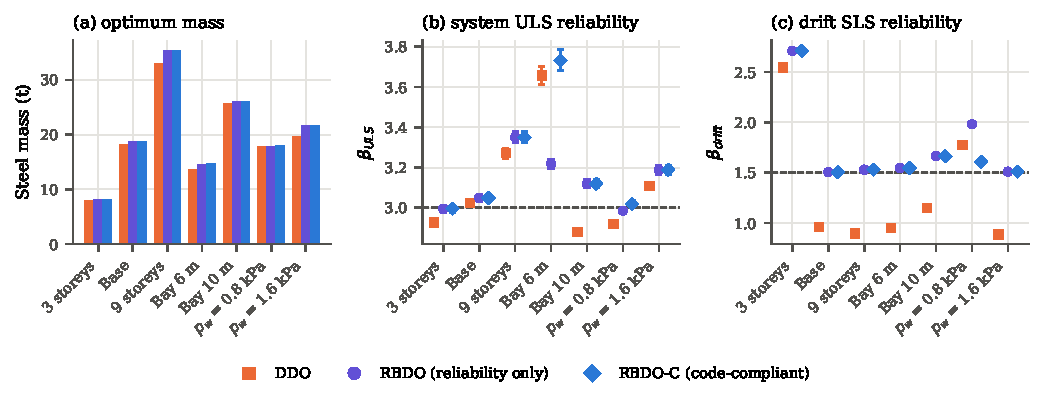
\includegraphics[width=\textwidth]{figures/parametric.pdf}
\caption{Parametric study: (a) optimum steel mass, (b) system ULS and (c) drift reliability
indices of the DDO and RBDO designs (independent $10^6$-sample verification); dashed lines
mark the targets.}
\label{fig:parametric}
\end{figure}

\subsection{Sensitivity to the probabilistic model}

Fig.~\ref{fig:sensitivity} shows how the verified reliability indices of the base designs
change when one assumption of Table~\ref{tab:rv} is altered ($4\times10^5$ samples each). The
system ULS index is most sensitive to the live-load model (c.o.v.\ 0.35 instead of 0.25:
$\Delta\beta\approx-0.5$), the fabrication factor (removing it: $+0.3$) and the yield-stress
model (mean-to-nominal 1.05 instead of 1.10, or c.o.v.\ 0.10 instead of 0.07: $-0.2$). Inter-member
correlation of $F_y$ changes $\beta_{ULS}$ by less than 0.05 in either direction, and the
out-of-plumbness and modulus variability are negligible. The drift index depends almost
exclusively on the wind model: a mean-to-nominal ratio of 0.90 instead of 0.78 lowers it by
0.4, and the c.o.v.\ changes it by about $\pm0.2$. The DDO and RBDO designs react in the same
way, so the conclusions of the comparison are robust to these assumptions, whereas the
\emph{absolute} indices, and hence the mass needed to meet a given target, are sensitive to the
live- and wind-load statistics. This is an argument for stating the probabilistic model
explicitly with any reliability-based design, as done here.

\begin{figure}[!htbp]
\centering
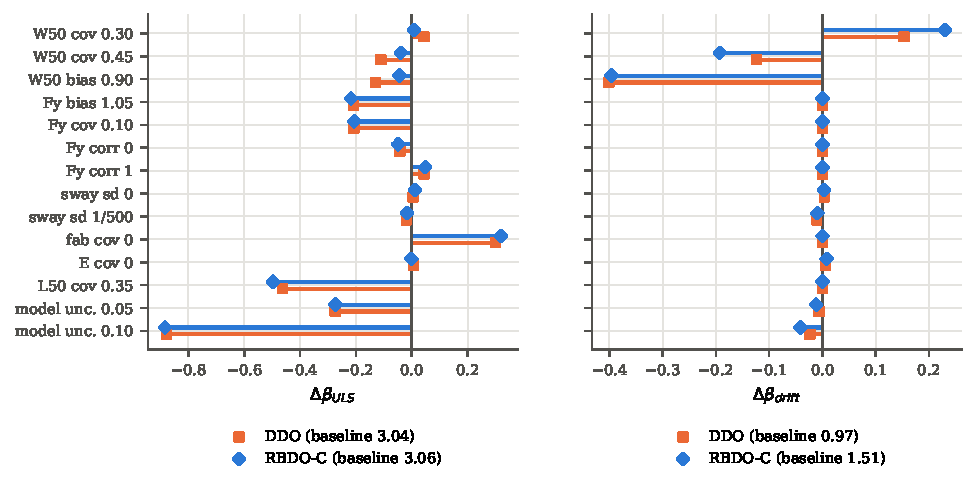
\includegraphics[width=\textwidth]{figures/sensitivity.pdf}
\caption{Change of the reliability indices of the base designs when one assumption of the
probabilistic model is changed (baseline indices in the legend).}
\label{fig:sensitivity}
\end{figure}

%% ---------------------------------------------------------------------------
\section{Discussion}\label{sec:discussion}

\paragraph{Answer to the research question}
For the frames studied, uncertainty-aware optimisation did \emph{not} produce lighter designs
than deterministic optimisation against the LRFD checks; it produced designs that were 0.5--10\%
heavier. The reason is not a weakness of RBDO but the fact that the deterministic optima are
already close to the reliability-based optimum for the ULS ($\beta_{ULS}\approx2.9$--3.7 at a
target of 3.0), while the conventional drift check at the nominal 50-year wind provides only
$\beta_{drift}\approx0.9$--1.2 for the drift-governed frames. When the reliability levels
implicit in the code are required, RBDO returns the DDO design exactly (Table~\ref{tab:targets}).
When a serviceability reliability of 1.5 is required, RBDO is the least-mass way of providing
it: it is never heavier than a deterministic design with a tightened drift limit that meets
the same targets, and it can trade surplus ULS reliability for stiffness. Economy is therefore
gained \emph{at a prescribed reliability}, not with respect to the code-based design, whose
reliability is unknown and non-uniform. Savings with respect to code-based designs can only be
expected where the code is conservative for the system considered, which in this study was
the case for the ULS of drift-governed frames (e.g.\ $\beta_{ULS}=3.66$ for 6-m bays) but was
masked by their serviceability deficit.

\paragraph{Cost of reliability}
The trade-off curves are strongly asymmetric. Once a frame is drift-governed, its ULS
reliability can be raised from 3.0 to almost 3.9 for about 4\% more steel
(Fig.~\ref{fig:pareto}), whereas the serviceability index is expensive to raise (2.9\% of steel to raise $\beta_{drift}$ from 0.96 to 1.51 in the base frame and 10.1\% from 0.89 to
1.51 in the high-wind frame).
Because the ULS and SLS indices of a given design are governed by different load scenarios
(Fig.~\ref{fig:memberutil}) and different random variables (Fig.~\ref{fig:sensitivity}),
a single global safety measure would hide these trade-offs; reporting both indices with
the mass, as done here, makes them explicit for owners and code writers.

\paragraph{Computational aspects}
The superposition surrogate is the enabling element of the framework. Five linear PyNite
analyses per design suffice to evaluate any number of load realisations and a global modulus
factor exactly, and the $B_1$--$B_2$ amplification added second-order effects within 2\% of
two independent P-$\Delta$ solvers. Full re-analysis Monte Carlo confirmed that ignoring
member-to-member stiffness variability and the stiffness effect of fabrication tolerances makes
the ULS estimate slightly conservative ($\approx1\%$ in utilisation). With common random numbers
the RBDO runs converge as robustly as the deterministic runs (identical optima for different GA
seeds). A three-objective NSGA-II run (mass, $\beta_{ULS}$, $\beta_{drift}$) with a comparable
budget of about 3500 designs did not approach the single-objective optima (its lightest design
with $\beta_{ULS}\ge3.0$ and $\beta_{drift}\ge1.5$ weighed 19.50~t against 18.79~t), so for
discrete frame problems of this size an $\varepsilon$-constraint approach with a strong
single-objective optimiser, complemented by a bi-objective front, is the more economical way
to map the trade-off.

\paragraph{Limitations}
The study considers regular planar moment frames with a single wind direction, a three-variable
grouping per storey group and a cost model proportional to steel mass; connection and
fabrication costs, which favour fewer distinct sections, are not included. The ULS is defined
by the first attainment of a member limit state in a second-order elastic analysis with the
AISC interaction equations, i.e.\ a code-format component criterion without inelastic
redistribution or model uncertainty of the interaction equations; system collapse
reliabilities obtained by advanced inelastic analysis \citep{Buonopane2006,Zhang2016} would be
higher. The live load on all floors and the frame-wide modulus are fully correlated, which is
conservative for the former. The load statistics are the classical ones of
\citet{Ellingwood1980}, and the mean-to-nominal ratio of $F_y$ is an assumption; the
sensitivity study shows that the absolute indices depend on these choices by up to
$\pm0.5$, although the comparison between DDO and RBDO does not. Finally, the drift SLS uses a
deterministic limit of $h/400$; a probabilistic drift capacity of non-structural components
\citep{Galambos1986} would refine the serviceability reliability.

%% ---------------------------------------------------------------------------
\section{Conclusions}\label{sec:conclusions}

A reproducible framework for reliability-constrained, multi-objective optimisation of steel
moment frames was developed on the open-source PyNite library and applied to a family of
planar frames with discrete W-shape sections. The main conclusions are:
\begin{enumerate}
\item Five linear PyNite analyses per design combined by superposition, with AISC $B_1$--$B_2$
amplification, give a reliability surrogate that agrees with OpenSeesPy to machine precision for
linear responses, within 2\% for P-$\Delta$ responses, and within about 1\% (conservatively)
with Monte Carlo simulation using full P-$\Delta$ re-analysis and member-by-member random
stiffness, at a cost that permits $5\times10^4$ samples per design inside a genetic algorithm.
\item Deterministic minimum-weight designs that satisfy the LRFD checks have non-uniform
reliability: system ULS indices between 2.88 and 3.66 and 50-year drift reliability indices
between 0.89 and 2.54 across the seven frames. Drift checked at the nominal 50-year wind
corresponds to $\beta_{drift}\approx1$ in drift-governed frames.
\item With targets of $\beta_T=3.0$ (ULS) and $\beta_{SLS}=1.5$, RBDO designs met both targets
in independent $10^6$-sample verification and were 0.5--10.1\% heavier than the deterministic
optima. When only the reliability levels implicit in the code were required, RBDO reproduced
the deterministic design exactly. Uncertainty-aware optimisation therefore did not yield more
economical designs than code-based optimisation for these frames; it yielded the least-mass
designs \emph{at an explicitly prescribed reliability}, and was never heavier than a
deterministic design with a tightened drift limit meeting the same targets, a limit which in
any case failed to meet them in two of five frames.
\item The cost--reliability trade-off is strongly asymmetric: in drift-governed frames the ULS
reliability index can be raised from about 3.0 to 3.8 for roughly 4\% more steel, while
raising the drift reliability index from 0.9--1.2 to 1.5 costs 1.7--10.1\%.
\item The absolute reliability indices are most sensitive to the live- and wind-load statistics
and to the yield-stress and fabrication models; the relative comparison of DDO and RBDO is
insensitive to them.
\end{enumerate}
Future work will extend the framework to three-dimensional frames, multiple wind directions
and seismic actions, a cost model including connections and fabrication, and inelastic system
limit states.
